\documentclass[10pt]{article}
\usepackage{tikz}
\usetikzlibrary{arrows.meta, positioning}

\usepackage{parskip}
\usepackage[margin=1in]{geometry} 
\usepackage{amsmath,amsthm,amssymb, graphicx, multicol, array}
\usepackage{enumitem}
\usepackage{amssymb}
\usepackage{float}
\usepackage{href-ul}
 
\newcommand{\N}{\mathbb{N}}
\newcommand{\Z}{\mathbb{Z}}
 
\newenvironment{problem}[2][Problem]{\begin{trivlist}
\item[\hskip \labelsep {\bfseries #1}\hskip \labelsep {\bfseries #2.}]}{\end{trivlist}}

\begin{document}
 
\title{Trends and Cycles I}
\author{Jakob Sverre Alexandersen\\
GRA4159 Trends, Cycles \& Signals Extraction\\
Lecture 6}
\maketitle

\tableofcontents
\newpage
\section{Recap}
\begin{itemize}
    \item Most macroeconomic data are time series --- thus we need to know about time series fundamentals
    \begin{itemize}
        \item The stationarity concept 
        \item Basic building blocks --- AR and MA 
    \end{itemize}
    \item A simple theory model helpful for making you think logically consistent about macroeconomic fluctuations 
    \begin{itemize}
        \item But variables are often framed as gaps (cycles), or at least stationary variables 
    \end{itemize}
    \item Most macroeconomic data are not stationary
    \begin{itemize}
        \item Different ``rules'' apply for data that is nonstationary 
    \end{itemize}
    \item Trends often make data nonstationary
    \begin{itemize}
        \item Removing the trend, or modelling the trend directly, allows us to use the stationary ``rules''
    \end{itemize}
    \item To do this correcly, it is important to separate between different trend processes:
    \begin{itemize}
        \item Deterministic trends 
        \item Stochastic trends 
    \end{itemize}
\end{itemize}
\subsection{Nonstationarity defined}
A time series process where either the first- or second-order moments (that is, mean and variance, respectively) depend on the time index is nonstationary
\section{Deterministic Trends}
\textbf{Definition:}

If a process includes $t $, it contains a deterministic trend 
\begin{itemize}
    \item consider the moving average process 
    \begin{gather*}
        y_t = \delta + \alpha t + \theta(L)\epsilon_t
    \end{gather*}
    where $\theta(L) = 1 + \theta_1L + \theta_2L^2 \dots $ and the deterministic trend is simply the time index $t $, with a slope parameter $\alpha $
    \item Including the trend, makes the process nonstationary:
    \begin{gather*}
        \mathbb{E}[y_t] = \delta + \alpha t
    \end{gather*}
    i.e., the mean depends on time 
    \item Note that deviations of $y_t $ from its mean are stationary:
    \begin{gather*}
        y_t - \mathbb{E}[y_t] = \delta + \alpha t + \theta(L)\epsilon_t - (\delta + \alpha t)\\
        = \theta(L)\epsilon_t
    \end{gather*}
    \item i.e., by removing the deterministic trend, the process becomes stationary
\end{itemize}
\newpage 
\section{Stochastic Trends}
\begin{itemize}
    \item The counterpart of a deterministic trend is a stochastic trend 
    \item The simplest model to think of with a stochastic trend is a Random Walk (RW): 
    \begin{gather*}
        y_t = y_{t - 1} + \epsilon_t \sim \text{i.i.d. }N(0, \sigma^2)
    \end{gather*}
\end{itemize}
\subsection{RW Properties}
\begin{itemize}
    \item Best forecast from an RW is: 
    \begin{gather*}
        \mathbb{E}[y_{t + 1}| y_t] = y_t 
    \end{gather*}
    \item The MSE of an RW grows linearly with the forecast horizon:
    \begin{gather*}
        \sigma_y(h) = \text{var}\big(y_{t + h} - \mathbb{E}[y_{t + h}|y_t]\big) = \sigma^2 h
    \end{gather*}
    \item Impulse response function for an RW does not return to zero. Shock persists forever 
\end{itemize}
\begin{figure}[H]
    \centering
    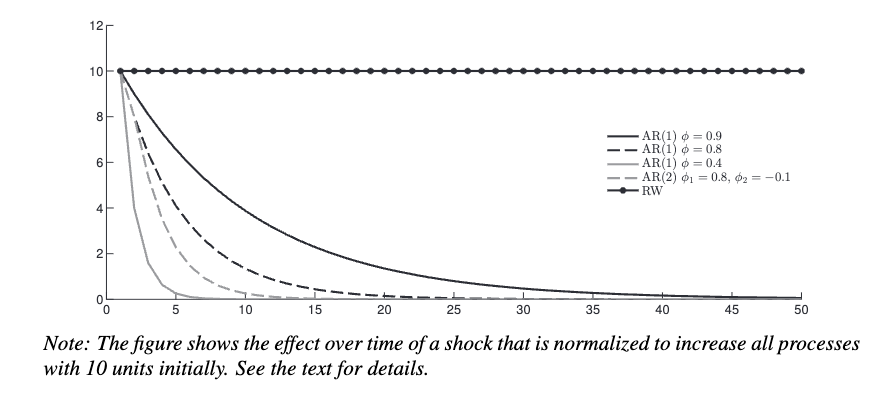
\includegraphics[width=0.8\textwidth]{2026-02-11-09-29-13.png}
\end{figure}
\begin{itemize}
    \item From previous discussions we know that RW is nonstationary. Can also show this by recursive substitution (assuming $y_0 = 0 $):
    \begin{gather*}
        y_t = y_{t - 1} + \epsilon_t\\
        = y_{t - 2} + \epsilon_{t - 1} + \epsilon_t\\
        \vdots\\
        y_t = \sum_{j = 0}^{t - 1}\epsilon_{t - j} + y_0\\
        y_t = \sum_{j = 0}^{t - 1}\epsilon_{t - j}
    \end{gather*}
    \item Accordingly, the variance of an RW depends on time: 
    \begin{gather*}
        \mathbb{E}[y_t] = 0\\
        \text{var}(y_t) = \sigma^2 t
    \end{gather*}
\end{itemize}
\newpage 
\subsection{Unit root}
\begin{itemize}
    \item The RW model can be made stationary simply by differencing the data: 
    \begin{gather*}
        y_t - y_{t - 1} = \epsilon_t\\
        \Delta y_t = \epsilon_t
    \end{gather*}
    clearly, $\Delta y_t $ is stationary
\end{itemize}
\textbf{Unit root defined}:
If variable $y_t $ can be made approximately stationary by differencing it once, we say that it is integrated of first order, $I(1) $, or that it has a unit root. Stationary random variables, such as $\Delta y_t $ are called integrated of order zero, $I(0) $.
\subsection{Random Walk with drift}
Can also add a constant to the RW: 
\begin{gather*}
    y_t = \alpha + y_{t - 1} + \epsilon_t
\end{gather*}
Then we get an RW with drift. The RW with drift can also be represented as a deterministic trend and stochastic term: 
\begin{gather*}
    y_t = \alpha + y_{t - 1} + \epsilon_t\\
    = \alpha + (y_{t - 2} + \alpha + \epsilon_{t - 1}) + \epsilon_t\\
    = 2\alpha(y_{t - 3} + \alpha + \epsilon_{t - 3}) + \epsilon_{t - 1} + \epsilon_t\\
    \vdots\\
    y_t = \alpha t + \sum_{j = 0}^{t -1}\epsilon_{t - j}
\end{gather*}
with $y_0 $ taken to be zero in the finite past. Compared to the simplest RW model, an RW with drift now also contains a deterministic trend. However, in contrast to the trend stationary model, the deviations from the deterministic trend are not stationary. 
\subsection{Trend stationarity and difference stationarity}
To remember: 
\begin{itemize}
    \item A series that returns to its trend after a shock is called trend stationary
    \item A series with a unit root is also called difference stationary
\end{itemize}
\begin{figure}[H]
    \centering
    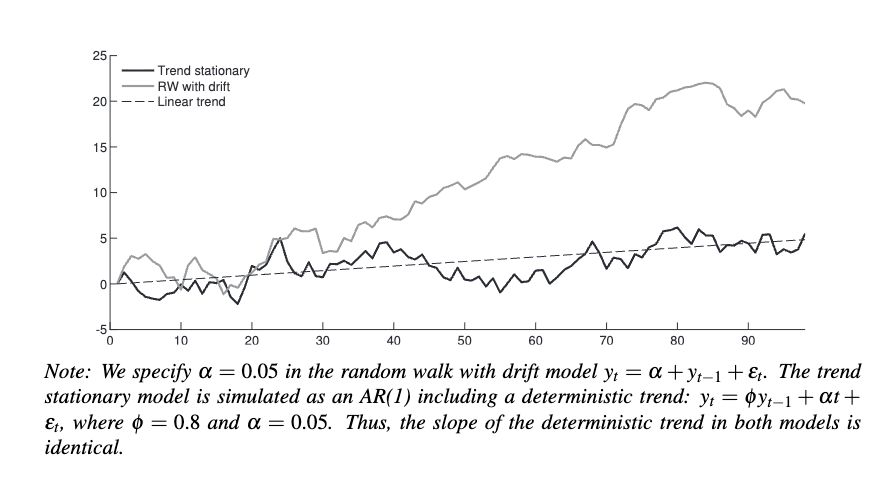
\includegraphics[width=0.7\textwidth]{2026-02-11-09-39-22.png}
\end{figure}
\newpage 
\section{Implications of Nonstationarity}
\begin{itemize}
    \item Normal ``rules'' do not apply. i.e., OLS regressions can give spurious results!
    \item Removing a deterministic trend from a series that has a stochastic model might induce spurious cycles in the data 
    \item If the data has a unit root, we can simply differences the data to make them stationary
    \item How can we test for unit roots?
\end{itemize}
\section{Tests for Unit Root --- The ADF Test}
\begin{itemize}
    \item Many tests do exist. Here: the Augmented Dickey Fuller (ADF) test. 
    \item Consider the following AR(1) process: 
    \begin{gather}
        y_t = \phi y_{t - 1} + \epsilon_t
    \end{gather}
    where $\epsilon_t \sim \text{i.i.d. }N(0, \sigma^2) $
    \item The question of interest is whether $\phi = 1 \text{ or }\phi < 1 $
    \begin{itemize}
        \item If $\phi = 1 $, equation (1) reduces to an RW 
        \item If $\phi < 1 $, the AR(1) process is stationary
    \end{itemize}
\end{itemize}
The ADF test: 
\begin{itemize}
    \item (1) can be rewritten as: 
    \begin{gather*}
        \Delta y_t = \mu y_{t - 1} + \epsilon_t
    \end{gather*}
    where $\mu = \phi - 1 $
    \item A test for a unit root is simply a test on the $\mu $ parameter, where: 
    \begin{gather*}
        H_0: \mu = 0 
    \end{gather*}
    which implies that $y_t $ is integrated of order one, $y_t\sim I(1) $, and the alternative:
    \begin{gather*}
        H_1 : \mu < 0 
    \end{gather*}
    which implies that $y_t $ is stationary, $y_t\sim I(0) $
    \item Can use $t $-statistic from the OLS estimate for $\mu $:
    \begin{gather*}
        \hat{t}_{\text{DF}} = \frac{\hat{\phi} - 1}{\text{SE}(\hat{\phi})} = \frac{\hat{\mu}}{\text{SE}(\hat{\mu})}
    \end{gather*}
    \item Note that the ADF test is one-sided and that asymptotic distribution for the $t $-value is non-Gaussian. i.e., we cannot use the critical values from the standard $t $-distribution
    \item It can also be shown that the OLS estimate of $\mu $ has a downward bias. Failing to correct for this bias, one is wrongly led to conclude that the series is stationary when it instead is an RW
\end{itemize}
\newpage 
\begin{itemize}
    \item Can include more lags to avoid autocorrelation in residuals
    \begin{gather*}
        y_t = \alpha + \phi_1y_{t - 1} + \phi_2y_{t - 2} + \epsilon_t
    \end{gather*}
    which is the same as: 
    \begin{gather*}
        \Delta y_t = \alpha + \mu y_{t - 1} + \gamma_1\Delta y_{t - 1} + \epsilon_t
    \end{gather*}
    \item Can include deterministic trend to control for drifts: 
    \begin{gather*}
        y_t = \alpha + \beta t + \phi y_{t - 1} + \epsilon_t
    \end{gather*}
    which can be rewritten as 
    \begin{gather*}
        \Delta y_t = \alpha + \beta t + \mu y_{t - 1} + \epsilon_t
    \end{gather*}
    where $\mu = \phi - 1 $, as above. Note that different critical values apply 
\end{itemize}
\begin{figure}[H]
    \centering
    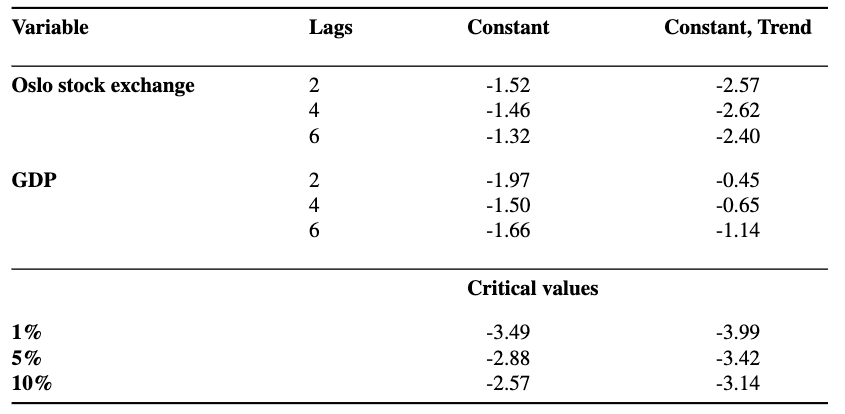
\includegraphics[width=0.7\textwidth]{2026-02-11-10-56-10.png}
\end{figure}
\begin{figure}[H]
    \centering
    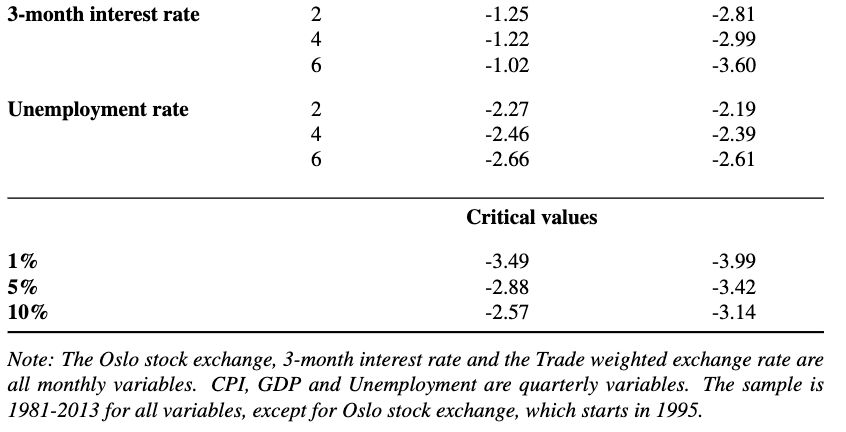
\includegraphics[width=0.7\textwidth]{2026-02-11-10-56-38.png}
\end{figure}
\newpage 
\section{Persistence}
An alternative method to analyze the degree of nonstationarity has been to analyze for how long macroeconomic variables respond to initial shocks. That is, how persistent are the effects of shocks to the time series?

Persistence implies that a shock lasts for a long time into the future. To measure this we start from the moving average representation of the first difference of a variable $y_t $. 

First, assume $y_t $ is nonstationary, but that the first-differences of the variable are stationary. Then $\Delta y_t $ has a moving average representation:
\begin{gather*}
    \Delta y_t = B(L)\epsilon_t = \epsilon_t + \beta_1\epsilon_{t - 1} + \beta_2\epsilon_{t - 2} + \dots
\end{gather*}
where $\beta_0 = 1 $, and as usual, $\epsilon_t \sim \text{i.i.d. } N(0, \sigma^2) $. Hence, $\Delta y_t $ is described entirely by its past and present shocks. $B(L) $ captures the impact of shocks over time. Put differently, the impact (or impulse response) of a shock in period $t $ on the \textit{growth rate} of $y $ in period $t + k $, is $B_k $. Thus, the impact of the same shock on the \textit{level} of $y $ at time $t + k $ is $1 + B_1 + \dots + B_k $

Finally, we have learned that the ultimate impact of a shock will be the infinite sum of the moving average coefficients (the cumululative effect of the shock), denoted $B(1) $: 
\begin{gather*}
    \sum_{j = 0}^{\infty}\frac{\partial y_{t + j}}{\partial \epsilon_t} = \sum_{j = 0}^{\infty}B_j\equiv B(1)
\end{gather*}
The value of $B(1) $ is the measure of persistence, as proposed by Campbell and Mankiw (1987). For an RW, $B(1) = 1 $, while for a stationary series (around a deterministic trend), $B(1) = 0 $. Hence, we can summarize: 
\begin{itemize}
    \item $B(1) = 1 $ for a random walk (shocks persist forever)
    \item $B(1) > 1 $, the ultimate effect is larger than the immediate effect (shocks explode)
    \item $B(1) < 1 $, the ultimate effect is less than the immediate eddect (shocks die out)
    \item $B(1) = 0 $ for a stationary series. 
\end{itemize}
How do we find $B(1)$= Assume $\Delta y_t $ follows an AR($p $) proces: 
\begin{gather*}
    \phi(L)\Delta y_t = \epsilon_t\\
    \Delta y_t = \frac{1}{\phi(L)}\epsilon_t \equiv B(L)\epsilon_t
\end{gather*}
Hence:
\begin{gather*}
    B(1) = \frac{1}{(1 - \theta_1 - \theta_2 - \dots - \theta_p)}
\end{gather*}
We have seen before that we can compute $B(1) $ for simple autoregressive models. For example, it was shown that for a stable AR(1), $B(1) = \frac{1}{1 - \phi} $. Thus, estimating an AR(1) on $\Delta y_t $ by OLS, will give us an estimate of $\phi $ and thereby also $B(1) $.
\newpage 
\begin{figure}[H]
    \centering
    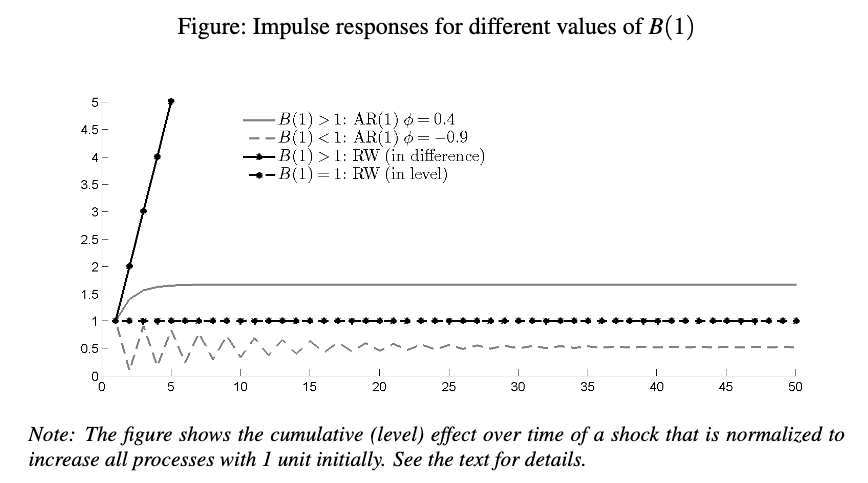
\includegraphics[width=0.8\textwidth]{2026-02-11-11-16-22.png}
\end{figure}
\section{Summary}
\begin{enumerate}
    \item A time series process where either the first- or second-order moments depend on the time index is nonstationary
    \item Time series having either a deterministic or stochastic trend are nonstationary
    \item If a process returns to its trent (some time) after a shock, we say that it is trend-stationary 
    \item Time series which are integrated of order one, $I(1) $, can be made stationary by simply differencing the time series. For this reason they are often called difference-stationary. Alternatively we say that they have one unit root 
    \item The simplest model containing a stochastic trend, and which is difference-stationary, is the random walk 
    \item Standard regression results as well as time series tools often rely on stationarity. Thus, it is important to test for nonstationarity: 
    \begin{itemize}
        \item Augmented Dickey-Fuller test (or other)
        \item Compute degree of persistence 
    \end{itemize}
\end{enumerate}
\end{document}